
\section{Compression of data}

This section will investigate the theory behind data compression, as well as trying to find compression techniques that could be used in the application. This study was requested by Thales.
\newline

Source coding, better known as data compression, is a way of reducing resource usage by compressing data. It performed on the data source before storing or transmitting the data. By encoding the data using fewer bits than the original representation the size of the data file decreases.

\begin{figure}[h!]
\begin{center}
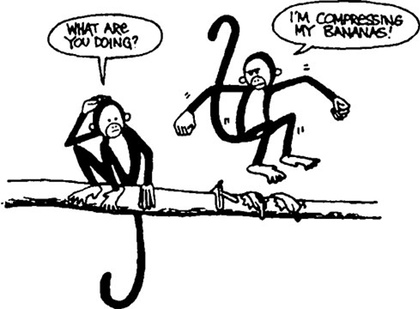
\includegraphics[scale=0.5]{compressionmonkeys}
\caption{There are many ways to compress ... \cite{bib:compressionImage}}
\end{center}
\end{figure}

\subsection{Benefits}
Compression is mainly used to reduce data storage space and transmission capacity. For the XOXOmail application both these features are important reasons to use data compression, but the most important is the one evolving transmission capacity. Since the users of the XOXOmail should be able to send pictures and videos as well as text, it is crucial to make the attachments as small as possible so that sending of a message with such attachments is possible, also in networks with poor bandwidth.

\subsection{Disadvantages}
Because that the data is compressed when receiving it, it must be decoded before use. This decoding is often resource demanding. Decoding of text and images are not very expensive and is done pretty fast.  When it comes to compressing and decompressing of video it is a quite different story. To encode a video without losing data is a time consuming task which requires expensive hardware. If the process is to slow, it will not be possible to watch the movie while it is being decoded. It is important to note that the result of decoding a compressed video may or may not give a different result thant the original data. This is dependent of the compression method used.

\pagebreak

\subsection{Data compression approaches}
There are two main ways to perform data compression. The two types are lossy and lossless data compression \cite{bib:dataCompression}. First we will describe lossy data compression as well as techniques for this method, then continue to do the same for lossless data compression.

\subsubsection{Lossy data compression}
Lossy compression means that data is lost during the compression procedure. When encoding the image, you do not get the original image out, because data is lost during the process. The purpose is to decrease the amount of data that must be sent or handled. Often the data, especially multimedia data, can be useful even though some of the data is lost, e.g. an image that will become coarser but still be very much like the full version. The compression algorithms often use well known properties of the human eye to remove details we cannot see. This makes it very hard to see the difference between a compressed and and uncompressed image. A well known usage of lossy compression is in streaming. There are two types of lossy compression approaches. \cite{bib:lossyCompression}

\paragraph{Lossy compression techniques for images}

\subparagraph{JPEG} \hfill
\newline
JPEG (Joint Photographic Experts Group) is an image format that uses a lossy compression method. The files usually get much smaller than when using image formats that use lossless compression methods. This format is often used for storing digital photos, especially photos for use on the Internet, because of the high compression rate. \cite{bib:JPEG}


\subparagraph{PGF} \hfill
\newline
The intention of Progressive Graphics File format was to improve and possibly replace the JPEG format. By using a wavelet-based image format, the compression is done with focus on speed over compression ratio. One of the benfits of compressing using PGF is that you can increase the compression ratio without using more time on the encoding. It also does not suffer from the compression artifacts that occurs in JPEG.
\cite{bib:PGF}

\paragraph{Lossy compression techniques for video}

\subparagraph{DV} \hfill
\newline
This was a format developed by the leading producers of video recorders. DV uses a lossy compression of the video, while the audio is stored uncompressed. The compression is done intra-frame, which means that each frame in the video is processed individually, not considering the frames in the sequence. The compression is done by a discrete cosine transform.
\cite{bib:DV}

\pagebreak

\subparagraph{MPEG} \hfill
\newline
The MPEG (Moving Picture Experts Group) compression is a bit more complicated than the DV scheme. Here, the frames are divided into I-, P- and B-frames. The I-frames are intra coded like in DV. The P-frames are forward predicted from the last I-frame or P-frame. They cannot be reconstructed alone. The B-frames are forward and backward predicted from one I-frame and one P-frame. B-frames and P-frames are therefore inter coded frames. The order of these frames are not sequential in the video, but the encoder ensures that the decoder gets the frames in the order required. After receival and processing, the frames need to be reordered before the video can be shown.
\cite{bib:MPEG}


\subparagraph{Dirac} \hfill
\newline
Dirac uses wavelet compression, just like PGF. It can be used with constant and variable bit rate, and when the low delay syntax is used, the bit rate will be constant for each area. This ensures constant latency. This makes it ideal for streaming.
\cite{bib:Dirac}


\subparagraph{VC-1} \hfill
\newline
VC-1 was initially developed by Microsoft, and is characterized as an alternative to the latest MPEG video encoding standard (H.264/MPEG-4 AVC). It contains tools for compression making it ideal for broadcast and video industry professionals. This, because of the ability to compress interlaced videos without first converting it to progressive.
\cite{bib:VC-1}


\paragraph{Lossy compression techniques for audio}


\subparagraph{MP3} \hfill
\newline
MP3 is shorthand for Moving Picture Experts Group, Audio Layer III, and is a compression method which is the common standard for most digital audio players. The encoding standard is a part of the MPEG-1 specification, and is vaguely defined. It is mostlly bitrate and sampling rate that is specified. The implementers can themself implement algorithms for removing parts of the information from the audio. It is only the decoder that is strictly specified.
\cite{bib:MP3}


\subparagraph{AAC}\hfill
\newline
AAC was designed to be the successor of the MP3 format. It is a part of the MPEG-2 and MPEG-4 standard. It will at the same bitrate as MP3 give better sound quality. The improvements are many, and some of them are variable bit-rates, more channels  and much better handling of audio frequencies above 16kHz.
\cite{bib:AAC}


\subparagraph{WMA} \hfill
\newline
Windows Media Audio is a proprietary compression technology developed by Microsoft. A WMA file is mostly within a container format which specifies how song name, track number, artist name, etc. are to be stored. It is in many ways similar to AAC, and its intent was also to replace the MP3 format.
\cite{bib:WMA}

\pagebreak

\subsubsection{Lossless data compression}
There will come, however, a point where lossy compression and decompression will have made the original data useless. Although the human eyes and ears may not catch small degradations of images and sounds, the decreased quality eventually will be apparent.
\newline
\newline
To have lossless compression means that the reconstruction of the compressed data is identical to the original data. A well-known example is the ZIP file format. Lossless compression is used when it is important that the original and decompressed data is identical, e.g. text or source code. The common way of doing lossless compression is to first generate a statistical model for the input data and secondly use this model to map input data to bit sequences. There are two ways of constructing statistical models. The first is to use static models, where data is analyzed and a model constructed, then the model is stored with the compressed data. This method is simple and modular, but the model can be expensive to store and the method may not perform well on files with heterogeneous data, as all data will have the same mode. The second method is to use an adaptive model. Here the model is dynamically updated as the data is compressed. The model is trivial at first but improves rapidly.
\newline
\newline
The most used encoding algorithms for producing bit sequences are Huffman coding and arithmetic coding. There are many special-purpose compression algorithms for e.g. images, text and video. In addition, there are many general-purpose lossless compression algorithms that may be used on any type of data. The problem arises when the input data is on another form than the algorithms were originally designed to compress.
A list of some common techniques and formats for lossless encodings will follow. \cite{bib:losslessCompression}


\paragraph{Lossless compression tecniques for text}

\subparagraph{Context tree weighting} \hfill
\newline
Is a lossless compression and prediction algorithm that is among the very few such algorithms that offer both theoretical guarantees and good practical performance. It uses variable order Markov models mixed together to make a context tree describing the data. \cite{bib:contextTreeWeighting} \cite{bib:contextTreeWeightingResearch}

\subparagraph{Burrows-Wheeler transform } \hfill
\newline
This is actually not an compression algorithm, but is often used on the data before it is compressed. The data amout after the transform is actually bigger, but it is transformed into a format that is more easily compressed by encoders. http://michael.dipperstein.com/bwt/index.html
\cite{bib:burrowsWheelerTransform}

\pagebreak

\subparagraph{LZ77} \hfill
\newline
LZ77 compress the data by looking for similar data occurences found earlier in the uncompressed data. The match is marked by saying how long the found occurence is from the data it matches. In this way, we dont't need to keep the same data later in the file, we just reference the location of the similar data. To keep the algorithm efficient, a sliding window defines the data we do matching on. If the sliding window is 32 kB, we only look back 32 kB to find a match.
\cite{bib:LZ77}

\paragraph{Lossless compression tecniques for images}
\subparagraph{GIF} \hfill
\newline
GIF ( Graphics Interchange Format) is an 8-bit-per-pikselbitmap-picture format used to store images. The format uses a palette of up to 256 colors from 24-bit RGB color space and are used extensively on the World Wide Web because the format is widely supported and easy to port. The format supports animation and allows separate palette of 256 colors for each frame. A GIF uses lossless compression so that the file size of an image can be reduced without changing the visual quality, as long as the image can be displayed with a maximum of 256 colors. \cite{bib:GIF} \cite{bib:gifSicle}

\subparagraph{PNG} \hfill
\newline
PNG (Portable Network Graphics) format has similarities with the GIF format, but contrary to GIF, the PNG-format is not limited to 256 colors for each frame. Each pixel in a PNG image may contain degrees of transparency. PNG format is best for images with large areas of identical color. \cite{bib:PNG}

\paragraph{Lossless compression tecniques for video}

\subparagraph{CorePNG} \hfill
\newline
Is a video compression codec, based on the PNG image compression format. Each frame is compressed as a PNG. The codec has the ability to write P-frames (prediction frames), thus saving the difference information from one image to the previous one. This significantly increases the compression, but requires more processing power and more memory for encoding and decoding. CorePNG is ideal for graphic videos, such as animation and CGI videos or desktop recordings, and for alpha channel video, so especially for films with relatively flat areas of color. \cite{bib:corePNG}

\subparagraph{Animation codec} \hfill
\newline
Animation codec is a QuickTimeCodec which is ideal for playback without expensive hardware.  This makes it very good for for example mobile devices. The Animation codec is very good on animation videos / videos where color changes are minor from frame to frame.
 \cite{bib:animationCodec}

\paragraph{Lossless compression techniques for sound}

\subparagraph{FLAC}\hfill
\newline
FLAC (Free Lossless Audio Codec) is a codec that has the ability to compress the audio signal with 50-60\%, depending on the content. This is an open format that has free licensing. The problem with compressing audio to flac format is that it is few portable devices that support the format. \cite{bib:FLAC}

\subparagraph{MPEG-4 SLS}\hfill
\newline
This is an extension to the MPEG-4 standard which enables lossless encoding of audio. The compression reached here is about 60\%. Licencing fees apply to using this codec, so it is not free to use like FLAC. \cite{bib:MPEGSLS}

\subsection{Discussion}
As we can see, there are two main methods for compression. What we can see from the previous sections, is that there exist a lot of methods for doing both lossy and lossless compression. Some of these methods are not so heavy, while others require a lot of processing power. The heaviest compression algorithms, processing wise, are those that operate on video streams. It is not trivial to compress images and text, but it is often very fast.

\paragraph{Choice of algorithms}\hfill
\newline
When choosing a compression algorithm, it is important to use a compression algorithm that gives good enough compression rate within the acceptable time frame. It is always good to compress data if the compression time is close to zero. This is seldom the case.
\newline
\newline
Often we do not know how good XOXOmail's connection to the Internet is. This can be calculated by taking the time it takes for data to be sent to / received from a server. If we then have some statistics on the compression time for, lets say 30 seconds of video, we can do some number crunching. If we know that with the current connection speed, the transfer of the compressed video will take 2 minutes to the mail server and 1 minute to get downloaded to the receiver (if assuming download rate is twice of upload, and that the receiver has the same connection as the sender) and it takes 20 seconds to check the connection speed, the total time used is then 3 minutes and 50 seconds. For the compression to be beneficial, the time used on compression and bandwith checking should be less than the time difference between sending and receiving the uncompressed and the compressed video.

\paragraph{Compressing text} \hfill
\newline
It is quite obvious that if we are to compress text sent via XOXO-mail, it has to be lossless. If we loose data on the way, the message received will look completely different than the one sent. This is not a result that we are interested in. One important thing to notice, is that the text size on the message sent via XOXOmail is often trivial. The sender often wants to convey a few sentences, together with the current coordinates and maybe an image. The text size compared to the image is negligble, so the effort of compressing the text is often not worth it. Of course, if we were to send large text files, then it would be another story.

\paragraph{Compressing images} \hfill
\newline
Compression of images is in this setting more resource demanding than compression of text, and can with good algorithms be compressed to 20 percent of original size, without too much degradation of the original content. Implementation of image compression methods are often compact and not so hard to implement. It is just a matter of finding the compression method which has the wanted end result.

\newpage

\paragraph{Compressing video} \hfill
\newline
Compression of video is one of the most resource demanding tasks that a phone can do. There exists a lot of algorithms for this, but unfortunately not so many for Android. Fortunately, it is a possiblity in Android to choose the video quality before starting to record the video. This can be done based on connection speed, but this does require that bandwidth is tested. This will result in creating a video with lower quality, so no compression has to be done. One must then do a judgement on how good video is good enough for showing what you intend to show via video. If the low settings of Android video is not good enough, then an algorithm needs to be used, either by a third party vendor or be implemented from scratch for Android. If a compression is chosen for getting wanted quality, then a choice on whether to use lossless or lossy compression also has to be made.

\paragraph{Compressing sound}\hfill
\newline
Compression of sound can be done with varying results. If you want to keep the original quality, lossless is the only alternative. There are a lot of alternatives for both lossy and lossless audio encoding. Some of them do not have licence fees, while others have. There exist some libraries that do what you want, but this of course depends on the format of the sound you are trying to send.

\subsection{Compression of data conclusion}
We have now gone through a lot of methods for both lossy and lossless compression and it is evident that there are many choices. The intention of this compression study was merely to give an overview of what exists. We have not listed all options, but just peeked into some of the most interesting methods. In order to give a qualified answer to what is the best algorithms, a more thorough study has to be done in order to find the requirements on compression time in relation with connection speed, what Android devices will be using the algorithms and what algorithms that have a working implementation for Android.  







